\begin{frame}{Zugfolge f�r $n=2$ und $k=3$}
\only<1>{
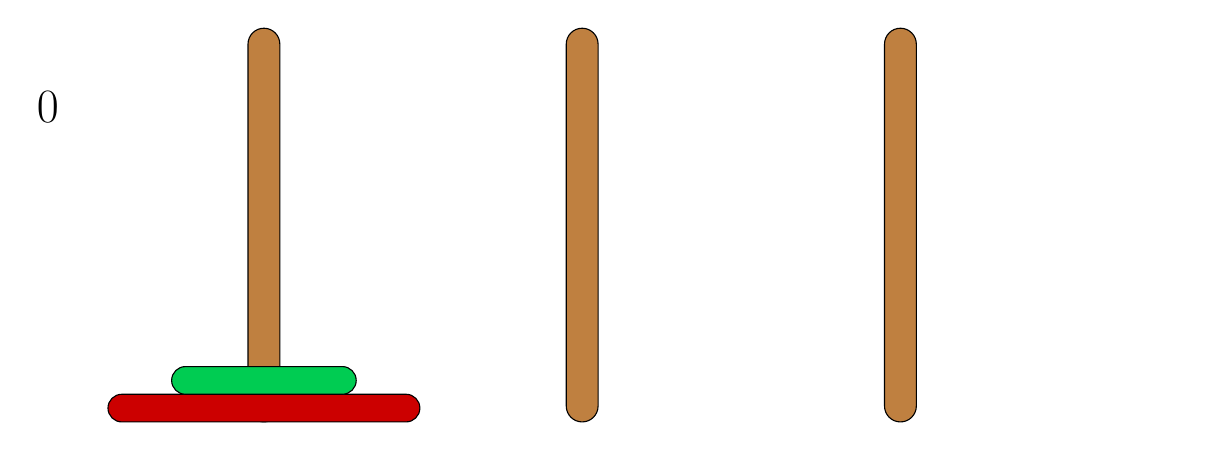
\begin{tikzpicture}
\pgfmathsetlengthmacro\diskheight{10};
\pgfmathsetmacro\k{3};
\pgfmathsetlengthmacro\step{\textwidth/\k};
\node[opacity = 1] at (1.5,4) {\LARGE 0};
\draw[color = white] (\step/2,0) -- (\textwidth+\step,0);
\foreach \n in {1,...,\k} \draw [fill = brown, draw = black, rounded corners = \step/20] (\step*\n,0) rectangle (\step*\n+\step/10,5);
\definecolor{mycolor}{rgb:hsb}{0.00,1,0.8}
\draw [fill = mycolor, draw = black, rounded corners = \diskheight/2] (\step*1+\step/20-\step*0.49,\diskheight*0) rectangle (\step*1+\step/20+\step*0.49,\diskheight*1);
\definecolor{mycolor}{rgb:hsb}{0.40,1,0.8}
\draw [fill = mycolor, draw = black, rounded corners = \diskheight/2] (\step*1+\step/20-\step*0.29,\diskheight*1) rectangle (\step*1+\step/20+\step*0.29,\diskheight*2);
\end{tikzpicture}
}
\only<2>{
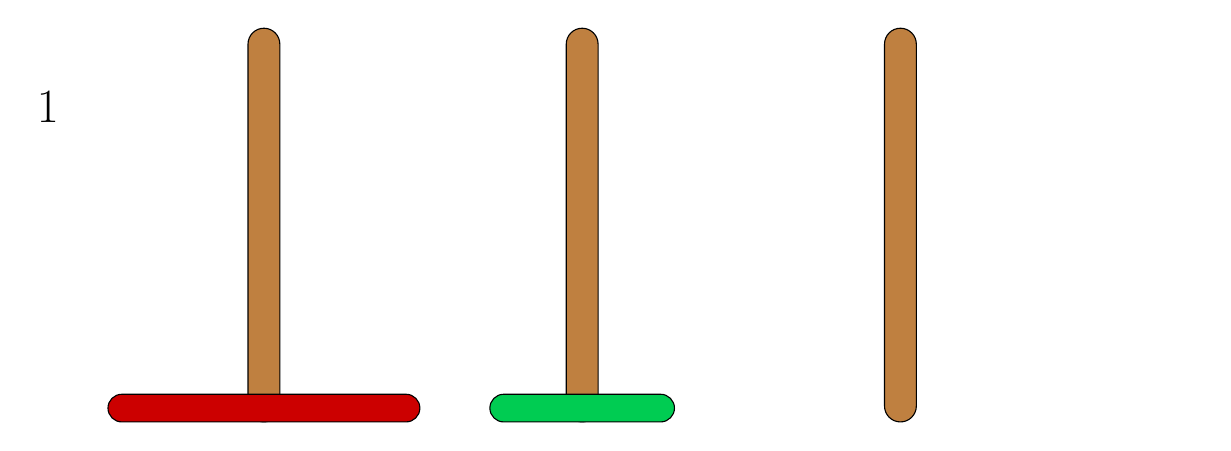
\begin{tikzpicture}
\pgfmathsetlengthmacro\diskheight{10};
\pgfmathsetmacro\k{3};
\pgfmathsetlengthmacro\step{\textwidth/\k};
\node[opacity = 1] at (1.5,4) {\LARGE 1};
\draw[color = white] (\step/2,0) -- (\textwidth+\step,0);
\foreach \n in {1,...,\k} \draw [fill = brown, draw = black, rounded corners = \step/20] (\step*\n,0) rectangle (\step*\n+\step/10,5);
\definecolor{mycolor}{rgb:hsb}{0.00,1,0.8}
\draw [fill = mycolor, draw = black, rounded corners = \diskheight/2] (\step*1+\step/20-\step*0.49,\diskheight*0) rectangle (\step*1+\step/20+\step*0.49,\diskheight*1);
\definecolor{mycolor}{rgb:hsb}{0.40,1,0.8}
\draw [fill = mycolor, draw = black, rounded corners = \diskheight/2] (\step*2+\step/20-\step*0.29,\diskheight*0) rectangle (\step*2+\step/20+\step*0.29,\diskheight*1);
\end{tikzpicture}
}
\only<3>{
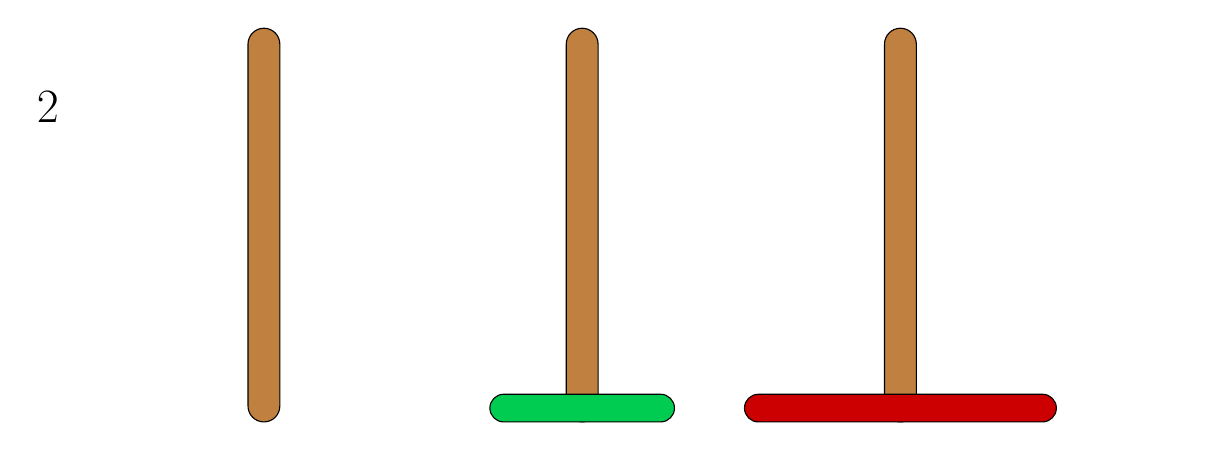
\begin{tikzpicture}
\pgfmathsetlengthmacro\diskheight{10};
\pgfmathsetmacro\k{3};
\pgfmathsetlengthmacro\step{\textwidth/\k};
\node[opacity = 1] at (1.5,4) {\LARGE 2};
\draw[color = white] (\step/2,0) -- (\textwidth+\step,0);
\foreach \n in {1,...,\k} \draw [fill = brown, draw = black, rounded corners = \step/20] (\step*\n,0) rectangle (\step*\n+\step/10,5);
\definecolor{mycolor}{rgb:hsb}{0.40,1,0.8}
\draw [fill = mycolor, draw = black, rounded corners = \diskheight/2] (\step*2+\step/20-\step*0.29,\diskheight*0) rectangle (\step*2+\step/20+\step*0.29,\diskheight*1);
\definecolor{mycolor}{rgb:hsb}{0.00,1,0.8}
\draw [fill = mycolor, draw = black, rounded corners = \diskheight/2] (\step*3+\step/20-\step*0.49,\diskheight*0) rectangle (\step*3+\step/20+\step*0.49,\diskheight*1);
\end{tikzpicture}
}
\only<4>{
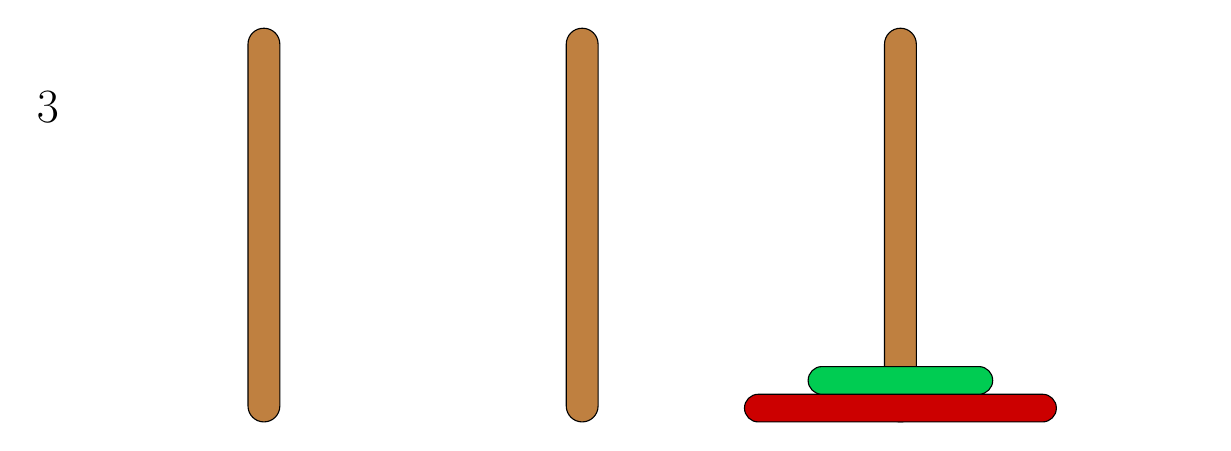
\begin{tikzpicture}
\pgfmathsetlengthmacro\diskheight{10};
\pgfmathsetmacro\k{3};
\pgfmathsetlengthmacro\step{\textwidth/\k};
\node[opacity = 1] at (1.5,4) {\LARGE 3};
\draw[color = white] (\step/2,0) -- (\textwidth+\step,0);
\foreach \n in {1,...,\k} \draw [fill = brown, draw = black, rounded corners = \step/20] (\step*\n,0) rectangle (\step*\n+\step/10,5);
\definecolor{mycolor}{rgb:hsb}{0.00,1,0.8}
\draw [fill = mycolor, draw = black, rounded corners = \diskheight/2] (\step*3+\step/20-\step*0.49,\diskheight*0) rectangle (\step*3+\step/20+\step*0.49,\diskheight*1);
\definecolor{mycolor}{rgb:hsb}{0.40,1,0.8}
\draw [fill = mycolor, draw = black, rounded corners = \diskheight/2] (\step*3+\step/20-\step*0.29,\diskheight*1) rectangle (\step*3+\step/20+\step*0.29,\diskheight*2);
\end{tikzpicture}
}
\end{frame}